% LaTeX Complete Guide: From Basics to Advanced Pro Level
% Save this file as `guide.tex` and compile with XeLaTeX or pdfLaTeX.

\documentclass[12pt,a4paper]{article}

% --------------------------------------------------
% 1. Package Imports (Core and Advanced)
% --------------------------------------------------
\usepackage[utf8]{inputenc}      % UTF-8 encoding
\usepackage[T1]{fontenc}         % Enhanced font encoding
\usepackage{lmodern}             % Latin Modern font
\usepackage{xcolor}              % Color support
\usepackage{geometry}            % Page margins
  \geometry{margin=1in}
  \usepackage{amsmath,amssymb,amsfonts,mathtools} % <-- ensures \mathbb and \boldsymbol work
\usepackage{graphicx}            % Image inclusion
\usepackage{hyperref}            % Hyperlinks
  \hypersetup{
    colorlinks=true,
    linkcolor=blue,
    urlcolor=cyan
  }
\usepackage[utf8]{inputenc}
\usepackage{newunicodechar}
\usepackage{pifont}
\newunicodechar{★}{\textcolor{teal}{\ding{72}}}
\usepackage{amsmath,amssymb,mathtools} % Math environments & symbols
\usepackage{bm}                  % Bold math symbols
\usepackage{unicode-math}        % Unicode math (with XeLaTeX/LuaLaTeX)
\usepackage{tikz}                % Graphics drawing
\usetikzlibrary{calc,intersections}
\usepackage[
backend=biber,
style=alphabetic,
sorting=ynt
]{biblatex}
\addbibresource{sample.bib}
\usepackage{pgfplots}            % Data plotting
  \pgfplotsset{compat=1.18}
\usepackage{tcolorbox}           % Colored boxes
  \tcbuselibrary{skins,breakable}
\usepackage{titlesec}            % Section formatting

% --------------------------------------------------
% 2. Colored Section Numbering with Special Character
% --------------------------------------------------
\titleformat{\section}
  [hang]
  {\normalfont\Large\bfseries}
  {\textcolor{teal}{★\thesection}}{1em}{}
\titleformat{\subsection}
  [hang]
  {\normalfont\large\bfseries}
  {\textcolor{violet}{◆\thesubsection}}{1em}{}

% --------------------------------------------------
% 3. Q&A Box Environments
% --------------------------------------------------
\newtcolorbox{questionbox}{
  colback=yellow!10, colframe=orange!70!black,
  title=Question, fonttitle=\bfseries
}
\newtcolorbox{answerbox}{
  colback=green!10, colframe=green!60!black,
  title=Answer, fonttitle=\bfseries
}

% --------------------------------------------------
% 4. Document Metadata
% --------------------------------------------------
\title{\LaTeX{} Complete Guide}
\author{Soham Bhadra}
\date{}

\begin{document}
\maketitle
\tableofcontents
\newpage

% --------------------------------------------------
% 5. Basics of a LaTeX Document
% --------------------------------------------------

\section{Introduction to LaTeX}

This guide is designed for absolute beginners who know nothing about LaTeX and takes you to advanced professional levels. It covers everything from basics to pro tips, including all mathematical symbols, image insertion, and more.

\begin{questionbox}
What is LaTeX?
\end{questionbox}

\begin{answerbox}
LaTeX is a typesetting system used for producing high-quality scientific and mathematical documents. It is not a word processor like Microsoft Word; instead, you write plain text with markup commands, and LaTeX compiles it into a PDF or other formats. It excels in handling complex math, references, and layouts.
\end{answerbox}

\begin{questionbox}
Why use LaTeX?
\end{questionbox}

\begin{answerbox}
LaTeX produces professional-looking documents, handles large documents easily, automates numbering and cross-references, and is free. It's standard in academia for papers, theses, and books.
\end{answerbox}

\begin{questionbox}
    How to Use LaTeX ?
\end{questionbox}

\begin{answerbox}
    Open Overleaf , create account and log in to your profile . Open a blank document and go to menu at top left corner , click it , change the compiler to XeLaTeX . Now let's get started .
\end{answerbox}
\begin{questionbox}
What are the essential elements of a LaTeX document?
\end{questionbox}
\begin{answerbox}
Every document must have a document class (e.g., \texttt{article}), preamble with package imports, and the \texttt{\textbackslash begin\{document\}} ... \texttt{\textbackslash end\{document\}} block.
\end{answerbox}

\subsection{Text Formatting}
\begin{itemize}
  \item \textbf{Bold text}: \texttt{\textbackslash textbf\{...\}}
  \item \textit{Italic text}: \texttt{\textbackslash textit\{...\}}
  \item \underline{Underline}: \texttt{\textbackslash underline\{...\}}
  \item \texttt{Monospaced}: \texttt{\textbackslash texttt\{...\}}
  \item Lists: \texttt{itemize}, \texttt{enumerate}, \texttt{description}
\end{itemize}

% --------------------------------------------------
% 6. Mathematics in LaTeX
% --------------------------------------------------
\section{Mathematical Environments}

\subsection{Inline and Display Modes}
Inline math: \( a^2 + b^2 = c^2 \). Display math:
\[
  e^{i\pi} + 1 = 0.
\]

\subsection{Common Symbols}
\begin{itemize}
  \item Greek letters: $\alpha,\beta,\gamma,\ldots,\Omega$.
  \item Operators: $\sum,\int,\prod,\lim,\sin,\cos,\log$.
  \item Relations: $=,\neq,\le,\ge,\approx,\equiv$.
  \item Arrows: $\rightarrow,\leftarrow,\Rightarrow,\leftrightarrow$.
  \item Delimiters: $( ),[ ],\{ \},\langle \rangle,\lvert \rvert,\lVert \rVert$.
  \item Accents: $\hat x,\bar x,\tilde x,\vec v$.
\end{itemize}

% --------------------------------------------------
% 7. Advanced Math Features
% --------------------------------------------------
\section{Advanced Mathematics}
\subsection{Aligned Equations and Modulos}

\begin{center}
    \[
    x+y=10
    \]
    \[
    2x-y=3
    \]
    \[
    2^{18}\equiv 1\pmod {19}\Longrightarrow (2^{18})^{96}\not\equiv 2\pmod{19}
    \]
\end{center}



\subsection{Symbols}
\begin{table}[h!]
  \centering
  \begin{tabular}{|c|c|c|c|c|c|}
    \hline
    $\clubsuit$ & $\spadesuit$ & $\blacksquare$ & $\heartsuit$ & $\infty$ & $\sqrt[n]{x}$ \\
    \hline
   $\triangle$ & $\hbar$ & $\Im$ & $\emptyset$ & $\nabla$ & $\mp$\\
    \hline
    $\mu$ & $\vartheta$ & $	\zeta$ & $	\chi$ & $\dagger$ & $\otimes$\\
    \hline
    
  \end{tabular}
  \caption{Symbols}
  \label{tab:simple}
\end{table}

Referencing equations: see Equation~\ref{eq:system}.

\subsection{More advanced Symbols}
\subsubsection{Integral}
\[
\int_{0}^{1} ln(x)=-1
\]

% Double integral over region D, triple over volume V, n‐fold over Ω
\[
  \iint\limits_D f(x,y)\,dx\,dy
  \quad,\quad
  \iiint\limits_V f(x,y,z)\,dV
  \quad,\quad
  \idotsint\limits_{g(x_1,x_2,\cdots,x_n)} f(x_1,\dots,x_n)\,dx_1\,dx_2\cdots dx_n.
\]

\subsubsection{Derivative}

% Second‑order and mixed partials, and general multi‑index notation
\[
  \frac{\partial^2 f}{\partial x^2}
  \quad,\quad
  \frac{\partial^2 f}{\partial x\,\partial y}
  \quad,\quad
  D^{\alpha}f
  = \frac{\partial^{|\alpha|}f}
         {\partial x_1^{\alpha_1}\,\partial x_2^{\alpha_2}\cdots\partial x_m^{\alpha_m}},
\]
where \(\alpha=(\alpha_1,\dots,\alpha_m)\) is a multi‑index and \(|\alpha|=\sum_{i=1}^m\alpha_i\).

\subsubsection{NT}

% p‑adic norm, canonical expansion in Z_p, and a Mahler‐series definition
\[
  |x|_p \;=\; p^{-\nu_p(x)},
  \quad
  x \;=\; p^{\nu_p(x)}\sum_{i=0}^\infty a_i\,p^i,
  \quad(a_i\in\{0,1,\dots,p-1\}).
\]
An analytic (continuous) function on \(\mathbb{Z}_p\) can be written via its Mahler expansion:
\[
  f(x) \;=\;\sum_{n=0}^\infty c_n\,\binom{x}{n},
  \quad
  c_n \;=\;\Delta^n f(0),
\]
where \(\binom{x}{n}=\tfrac{x(x-1)\cdots(x-n+1)}{n!}\) and \(\Delta^n\) is the finite‐difference operator.

\subsubsection{Putnam 2003 B3}

Show that for each positive integer n,\[n!=\prod_{i=1}^n \; \text{lcm} \; \{1, 2, \ldots, \left\lfloor\frac{n}{i} \right\rfloor\}\](Here lcm denotes the least common multiple, and $\lfloor x\rfloor$ denotes the greatest integer $\le x$.)


\subsection{Matrices and Cases}
\[
  \begin{pmatrix}
    a & b \\
    c & d
  \end{pmatrix},
  \quad
  f(x)=
  \begin{cases}
    x^2 & x\ge0,\\
    -x  & x<0.
  \end{cases}
\]

% --------------------------------------------------
% 8. Including Graphics
% --------------------------------------------------
\section{Figures and Tables}
\subsection{Image Insertion}
\begin{figure}[h!]
  \centering
  \includegraphics[width=0.5\textwidth]{LaTeX_logo.svg.png}
  \caption{An Example Image}
  \label{fig:example}
\end{figure}

\subsection{Tables}
\begin{table}[h!]
  \centering
  \begin{tabular}{|c|c|c|}
    \hline
    A & B & C \\
    \hline
    1 & 2 & 3 \\
    \hline
    4 & 5 & 6 \\
    \hline
  \end{tabular}
  \caption{Simple Table}
  \label{tab:simple}
\end{table}

% --------------------------------------------------
% 9. TikZ and PGFPlots for Graphics
% --------------------------------------------------
\section{Drawing and Plotting}
\subsection{Basic TikZ Illustration}
\begin{tikzpicture}
  \draw[->,thick] (0,0) -- (3,0) node[right]{$x$};
  \draw[->,thick] (0,0) -- (0,3) node[above]{$y$};
  \draw[blue,domain=0:2.5] plot(\x,\x^2);
\end{tikzpicture}

\subsection{Plotting Data}
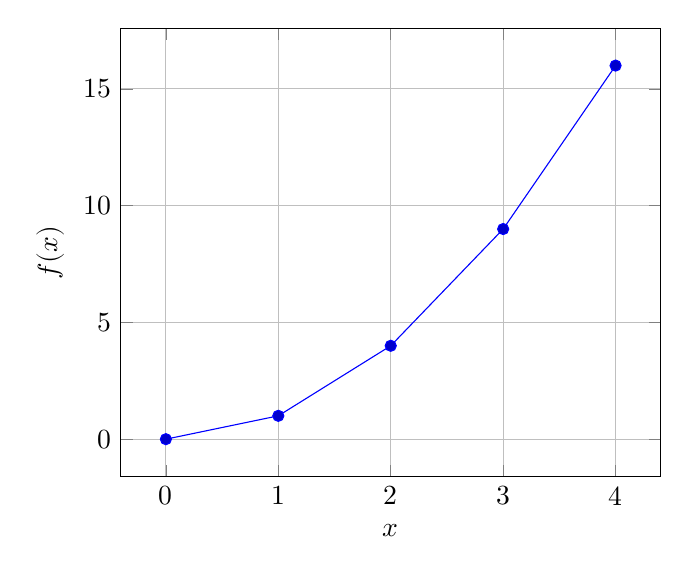
\begin{tikzpicture}
\begin{axis}[xlabel=$x$,ylabel={$f(x)$},grid=both]
  \addplot table[col sep=comma]{
    x,y
    0,0
    1,1
    2,4
    3,9
    4,16
  };
\end{axis}
\end{tikzpicture}

\section{Customization}

\subsection{Custom Environments}
\newenvironment{theorem}[1][]{
  \begin{tcolorbox}[colback=blue!5,colframe=blue!70!black,title=Theorem #1]
}{
  \end{tcolorbox}
}

\begin{theorem}[Pythagoras]
In a right triangle, $a^2 + b^2 = c^2$.
\end{theorem}

% --------------------------------------------------
% 11. Bibliography with BibLaTeX
% --------------------------------------------------
\section{References}
Let's cite! Einstein's journal paper \cite{einstein} and Donald Knuth \cite{knuth} are physics-related items. 

\printbibliography %Prints bibliography
\printbibliography

@article{einstein,
    author = "Albert Einstein",
    title = "{Zur Elektrodynamik bewegter K{\"o}rper}. ({German})
    [{On} the electrodynamics of moving bodies]",
    journal = "Annalen der Physik",
    volume = "322",
    number = "10",
    pages = "891--921",
    year = "1905",
    DOI = "http://dx.doi.org/10.1002/andp.19053221004",
    keywords = "physics"
}

@online{knuthwebsite,
    author = "Donald Knuth",
    title = "Knuth: Computers and Typesetting",
    url  = "http://www-cs-faculty.stanford.edu/~uno/abcde.html"
}


% --------------------------------------------------
% 12. Document End
% --------------------------------------------------
\end{document}